\documentclass[11pt]{ctexart}

\usepackage{geometry}
\geometry{
    left = 0.6in,
    right = 0.6in,
    top = 0.8in,
    bottom = 1.0in
}
\usepackage{amssymb,amsbsy,amsmath,xcolor,mathrsfs,graphicx}
\usepackage{listings}
\usepackage{tasks}
\settasks{
    label = \Alph*. ,
    label-width = 16pt
}

\renewcommand{\title}[3]{
    \begin{center}
        \Large\heiti 中国电子学会 #1~年~#2~月 Python~#3级考试
    \end{center}
}
\newcommand{\TimeAndName}[1]{
    \begin{center}
        考试时间:~#1~ 分钟 \qquad\qquad\qquad\qquad 姓名:\underline{\quad\quad\quad\quad}
    \end{center}
}

\begin{document}
    \lstset{
        language = python,
        keywordstyle = \color{orange}\bfseries,
        emph = {
            abs, all, any, ascii, bin, bool, breakpoint, bytearray, bytes,
            callable, chr, classmethod, compile, complex, copyright, credits,
            delattr, dict, dir, divmod, enumerate, eval, exec, exit, filter,
            float, format, frozenset, getattr, globals, hasattr, hash,
            help, hex, id, input, int, isinstance, issubclass, iter, len,
            license, list, locals, map, max, memoryview, min, next, object,
            oct, open, ord, pow, print, property, quit, range, repr, reversed,
            round, set, setattr, slice, sorted, staticmethod, str, sum, super,
            tuple, type, vars, zip,
        },
        emphstyle = \color{purple}\bfseries,
        showspaces = false,
        basicstyle = \ttfamily,
        morekeywords = {True,False}
    }

    \title{2021}{6}{一}
    
    \TimeAndName{60}
    
    {\noindent\heiti 第一部分、单选题(共 25 题,每题 2 分,共50分.)}

    \begin{enumerate}
        % 1
        \item 下列哪个操作不能退出 IDLE 环境?(\qquad)
        \begin{tasks}(4)
            \task Alt + F4
            \task Ctrl + Q
            \task 按 ESC 键
            \task \lstinline{exit()}
        \end{tasks}
    

        % 2
        \item \lstinline!print(4 + 8 // 2)! 的输出结果是?(\qquad)
        \begin{tasks}(4)
            \task 6
            \task 6.0
            \task 8
            \task 8.0
        \end{tasks}

        % 3
        \item 下列哪个软件不能进行 Python 代码编写?(\qquad)
        \begin{tasks}(4)
            \task IDLE
            \task PyCharm
            \task Visual~Studio~Code
            \task WPS
        \end{tasks}
    
        % 4
        \item 下列哪个符号可以用来修改变量的值?(\qquad)
        \begin{tasks}(4)
            \task \lstinline{>=}
            \task \lstinline{<=}
            \task \lstinline{==}
            \task \lstinline{=}
        \end{tasks}

        % 5
        \item 关于\lstinline!print()!语句,下列选项能够正确输出的是?(\qquad)
        \begin{tasks}(2)
            \task \lstinline{print('hello!,2021年!')}
            \task \lstinline{print 'hello!,2021年!'}
            \task \lstinline{print"(hello!,2021年!)"}
            \task \lstinline{print("hello!,2021年!')}
        \end{tasks}

        % 6
        \item 运行下列代码,\lstinline{d} 输出的结果是?(\qquad)
        \begin{lstlisting}
            a, b, c = 23, 13, 3
            d = (a + b) - c * c
        \end{lstlisting}
        \begin{tasks}(4)
            \task 22
            \task 27
            \task 99
            \task 9
        \end{tasks}

        % 7
        \item 下列代码段的结果是?(\qquad)
        \begin{lstlisting}
            star_number1 = "star2"
            star_number2 = "star3"
            print(star_number1 + star_number2)
        \end{lstlisting}
        \begin{tasks}(4)
            \task \lstinline{star5}
            \task \lstinline{star3star2}
            \task \lstinline{star2star3}
            \task \lstinline{star23}
        \end{tasks}

        % 8
        \item Python中的余数运算符是用哪个符号表示的?(\qquad)
        \begin{tasks}(4)
            \task \%
            \task /
            \task //
            \task \lstinline!\\\\!
        \end{tasks}

        % 9
        \item 下列运算中,运算结果为 \lstinline!True! 的是?(\qquad)
        \begin{tasks}(4)
            \task \lstinline!2>3 and 3>2!
            \task \lstinline{4=!0 and 3+2>=5}
            \task \lstinline!3**2<8 or 3+2<5!
            \task \lstinline!not 20>=20!
        \end{tasks}

        % 10
        \item 在turtle库中的指令,执行以下代码指令后,画笔为以下哪种状态?(\qquad)
        \begin{lstlisting}
            import turtle
            turtle.color('pink')
            turtle.pensize(5)
        \end{lstlisting}
        \begin{tasks}(2)
            \task 画笔颜色为粉色,画笔宽度为5
            \task 画笔颜色为黄色,画笔宽度为5
            \task 画布背景为粉色,画笔宽度为5
            \task 画笔颜色为粉色,画笔速度为5
        \end{tasks}

        % 11
        \item 下列代码的运行结果是?(\qquad)
        \begin{lstlisting}
            import turtle
            turtle.color('red')
            turtle.circle(100)
            turtle.fillcolor('yellow')
            turtle.begin_fill()
            turtle.circle(100,steps = 6)
            turtle.end_fill()
        \end{lstlisting}
        \begin{tasks}(4)
            \task 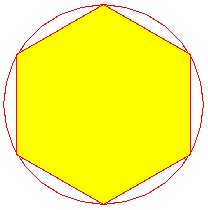
\includegraphics[width=.1\textwidth]{11a.png}
            \task 
\includegraphics[width=.1\textwidth]{11b.png}
            \task 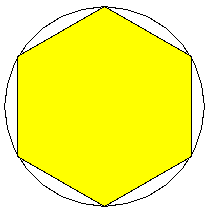
\includegraphics[width=.1\textwidth]{11c.png}
            \task 
\includegraphics[width=.1\textwidth]{11d.png}
        \end{tasks}

        % 12
        \item 下列哪一段代码是海龟走到指定坐标然后左转90度?(\qquad)
        \begin{tasks}(4)
            \task \lstinline!turtle.goto(90,0)! \\ \lstinline!turtle.left(90)!
            \task \lstinline!turtle.left(90)! \\ \lstinline!turtle.goto(90,0)!
            \task \lstinline!turtle.goto(90,0)! \\ \lstinline!turtle.right(90)!
            \task \lstinline!turtle.right(90)! \\ \lstinline!turtle.goto(90,0)!
        \end{tasks}

        % 13
        \item 下列关于turtle库的描述不正确的是?(\qquad)
        \begin{tasks}(2)
            \task 画笔的初始坐标为(0,0)
            \task turtle.color()可以设置画笔的颜色
            \task 画笔绘制的速度没有范围
            \task turtle.fillcolor()设置绘制图形的填充颜色
        \end{tasks}

        % 14
        \item 同学们排队做操,按名单顺序,每10个人一排,要问第n个人是第几排,下列哪一种方法可以实现?(\qquad)
        \begin{tasks}(4)
            \task \lstinline!n//10!
            \task \lstinline!n\%10!
            \task \lstinline!(n-1)//10+1!
            \task \lstinline!(n-1)\%10+1!
        \end{tasks}
        
        % 15
        \item 在Python IDLE中输入\lstinline!print('Hello');print('I am Python');!,并将这两个语句写在一行,试分析,程序的运行结果是以下哪个选项?(\qquad)
        \begin{tasks}(4)
            \task \lstinline!Hello!
            \task \lstinline!I am Python!
            \task \lstinline!Hello! \\ \lstinline!I am Python!
            \task 语法错误
        \end{tasks}

        \newpage
        % 16
        \item 下列哪个命令可以将整个绘制屏幕的颜色设置成黑色?(\qquad)
        \begin{tasks}(2)
            \task \lstinline!turtle.screensize("black")!
            \task \lstinline!turtle.fillcolor("black")!
            \task \lstinline!turtle.bgcolor("black")!
            \task \lstinline!turtle.pencolor("black")!
        \end{tasks}

        % 17
        \item 执行\lstinline!print(3>2 or 4<5)!的结果是?(\qquad)
        \begin{tasks}(4)
            \task 1
            \task 0
            \task True
            \task False
        \end{tasks}

        % 18
        \item 下列哪个选项的运算优先级最高?(\qquad)
        \begin{tasks}(4)
            \task \lstinline{==}
            \task \lstinline{*}
            \task \lstinline{and}
            \task \lstinline{+}
        \end{tasks}

        % 19
        \item 为变量命名,并赋值为数字1,以下选项中,不符合要求的是?(\qquad)
        \begin{tasks}(4)
            \task \lstinline!abc = 1!
            \task \lstinline!HelloWorld = 1!
            \task \lstinline!1abc = 1!
            \task \lstinline!abc_xyz = 1!
        \end{tasks}

        % 20
        \item 已知变量a = 5,执行下列哪个代码后,a的值为10?(\qquad)
        \begin{tasks}(4)
            \task \lstinline!a >= a + 5!
            \task \lstinline!a += a + 5!
            \task \lstinline!a == a + 5!
            \task \lstinline!a *= a + 5!
        \end{tasks}

        % 21
        \item 下列可以用作多行注释的是?(\qquad)
        \begin{tasks}(4)
            \task 前后加 \lstinline!//!
            \task 前后加 \lstinline!\'\'\'!
            \task 前后加 \lstinline!***!
            \task 前后加 \lstinline!\#\#\#!
        \end{tasks}

        % 22
        \item \lstinline!turtle.circle(90, 180)!是绘制一个什么样的图形?(\qquad)
        \begin{tasks}(4)
            \task 半径为180的扇形
            \task 半径为90的半圆
            \task 半径为90的圆形
            \task 半径为180的圆形
        \end{tasks}

        % 23
        \item 下列代码执行后最有可能绘制出哪个图形?(\qquad)
        \begin{lstlisting}
            import turtle
            turtle.forward(100)
            turtle.right(90)
            turtle.forward(100)
            turtle.right(45)
            turtle.goto(0,0)
            turtle.hideturtle()
        \end{lstlisting}
        \begin{tasks}(4)
            \task 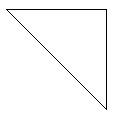
\includegraphics[width=.1\textwidth]{23a.png}
            \task 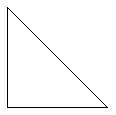
\includegraphics[width=.1\textwidth]{23b.png}
            \task 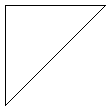
\includegraphics[width=.1\textwidth]{23c.png}
            \task 
\includegraphics[width=.1\textwidth]{23d.png}
        \end{tasks}

        \newpage
        % 24
        \item 关于Python,下列哪个表述是正确的?(\qquad)
        \begin{tasks}
            \task Python只可以在windows系统中使用
            \task 在Windows系统中编写的程序不可以在Linux或者IOS系统中打开
            \task Python目前存在Python 2 和Python 3 两个版本,但并不完全兼容
            \task 32位的电脑系统可支持安装64位版本的Python软件
        \end{tasks}

        % 25
        \item \lstinline!print(6+8/2)!输出的结果是?(\qquad)
        \begin{tasks}(4)
            \task 7
            \task 10.0
            \task 10
            \task 7.0
        \end{tasks}
    \end{enumerate}

    {\noindent\heiti 第二部分、判断题(共 10 题,每题 2 分,共20分.)}
    \begin{enumerate}
        \setcounter{enumi}{25}
        % 26
        \item 以下三种表示字符串的方式都是正确的(\qquad)
        \begin{lstlisting}
            "Hello"
            '不错'
            "我们一起走吧'
        \end{lstlisting}

        %27
        \item 设置画布背景颜色只有 \lstinline!turtle.bgcolor()! 一种方法(\qquad)
        
        %28
        \item 在IDLE中,要新建Python脚本,在菜单里可以依次选择File->New File 即可新建Python脚本(\qquad)
  
        %29
        \item 在用IDLE脚本方式编写程序时,可以用ctrl+s快捷键保存代码(\qquad)
        
        %30
        \item 12number、my~number、my\_number都是有效的变量名(\qquad)
        
        %31
        \item 在Python的编程环境中,缩进的空格数是可以改变的,同一个代码块可以有不相同的缩进空格数(\qquad)
        
        %32
        \item 每一个变量在使用前都必须赋值,赋值以后该变量才会被创建(\qquad)
        
        %33
        \item  Turtle库属于图形绘制函数库(\qquad)
        
        %34
        \item 在Python中,编程语言是不区分大小写的,如: \lstinline{print()} 是打印函数,\lstinline{Print()} 也是打印函数(\qquad)
        
        %35
        \item 以下代码可以计算出2030年时的年龄(\qquad)
        \begin{lstlisting}
            year = input("请输入您的出生年份:")
            print("到了2030年,您的年龄是:", 2030-year)
        \end{lstlisting}
    \end{enumerate}

    \newpage
    {\noindent\heiti 第三部分、编程题(共 2 题,共30分.)}
    \begin{enumerate}
        \setcounter{enumi}{35}
        
        % 36
        \item 绘制如下图形,一个正方形,内有三个红点,中间红点在正方形中心.要求如下:
        \begin{figure}[htbp]
            \begin{minipage}{.68\textwidth}
                \begin{tasks}[label=(\arabic*)]
                    \task 正方形边长为200,线条为黑色;
                    \task 圆点的直径均为20 ,填充颜色为红色,画完后隐藏画笔;
                    \task 中间圆点的圆心位置为画布正中心,三个圆心之间距离相隔为40.
                \end{tasks}
            \end{minipage}
            \begin{minipage}{.3\textwidth}
                \centering
                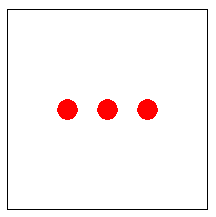
\includegraphics[width=.4\textwidth]{36.png}
            \end{minipage}
        \end{figure}
        \vfill

        %37
        \item 写一个计算长方形面积的程序,并对每行代码进行相应的注释,要求如下:
        
        \begin{tasks}[label=(\arabic*)]
            \task 采用多行注释,说明程序的功能(如下):
            
            “计算长方形的面积
            
            并输出结果”;

            \task 设置第1个变量:用“a”表示长方形的长,并赋值为6;使用单行注释说明程序的功能;
            \task 设置第2个变量:用“b”表示长方形的宽,并赋值为3;使用单行注释说明程序的功能;
            \task 设置第3个变量:用“s”表示长方形的面积,并体现运算公式,使用单行注释说明程序功能;
            \task 输出长方形的面积,运行结果格式为:“长方形的面积为:”并使用单行注释说明程序功能。
        \end{tasks}
        \vfill
    \end{enumerate}
\end{document}